\title{Mapping Scientific Activity in Enlightenment Period Latin America}
\author{Dr. Jordan Hanson - Whittier College Dept. of Physics and Astronomy}
\date{\today}
\documentclass[12pt]{article}
\usepackage[margin=1.25cm]{geometry}
\usepackage{hyperref}
\usepackage{graphicx}
\usepackage{amsmath}
\usepackage{subcaption}
\begin{document}
\maketitle

\small

\section{Introduction}

\begin{figure}[ht]
\centering
\begin{subfigure}{0.125\textwidth}
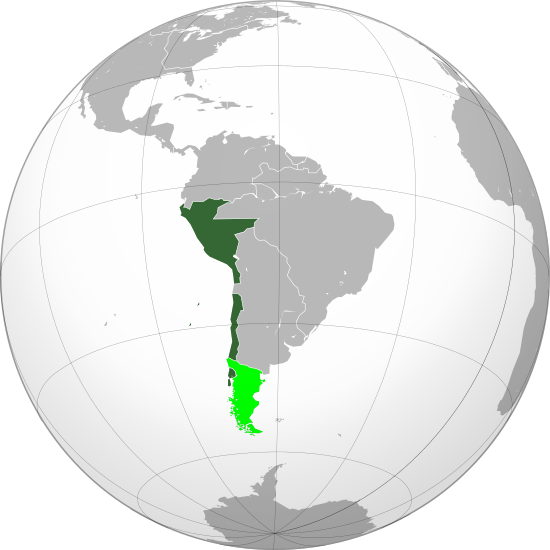
\includegraphics[width=\textwidth]{vice_peru.png}
\caption{\label{fig:1a}}
\end{subfigure}
\begin{subfigure}{0.125\textwidth}
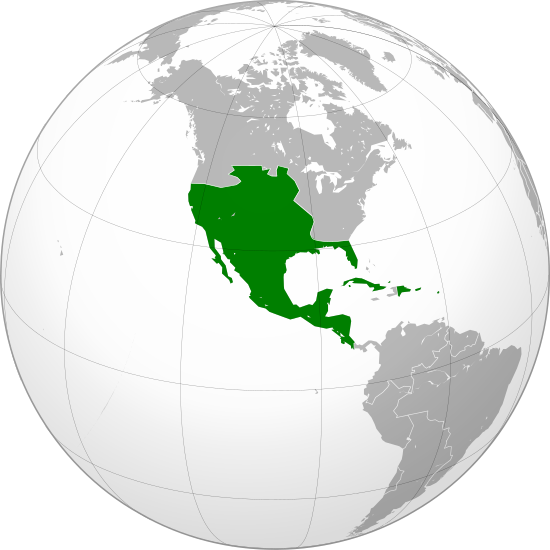
\includegraphics[width=\textwidth]{vice_nuevaespana.png}
\caption{\label{fig:1b}}
\end{subfigure}
\begin{subfigure}{0.125\textwidth}
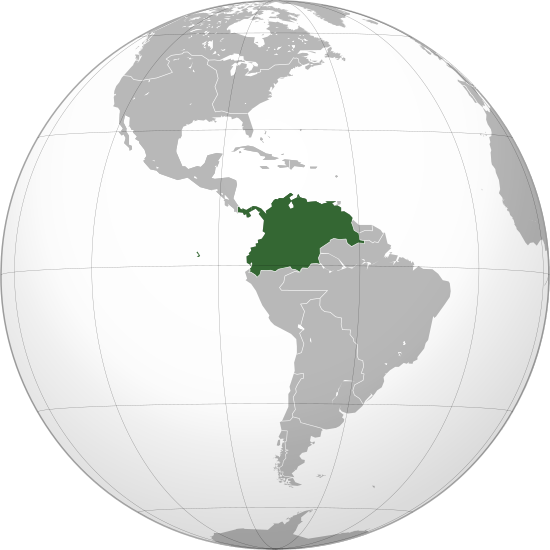
\includegraphics[width=\textwidth]{vice_nuevagranada.png}
\caption{\label{fig:1c}}
\end{subfigure}
\begin{subfigure}{0.125\textwidth}
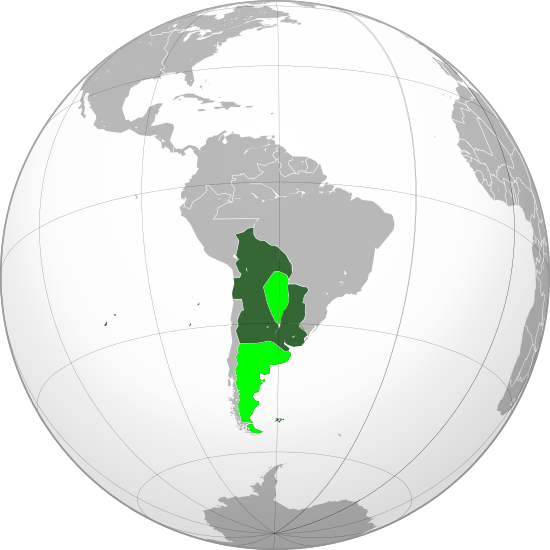
\includegraphics[width=\textwidth]{vice_riodelaplata.png}
\caption{\label{fig:1d}}
\end{subfigure}
\caption{\label{fig:1} Maps depicting \textit{virreinatos} in Latin America, 17th and 18th centuries.}
\end{figure}

In chapters 2 and 3 of \textit{Science in Latin America}, we see examples of the importation of scientific texts, the creation of scientific journals, the creation of \textit{Sociedades de los Amigos del Pa\'{i}s} (and other secular groups), the founding of colleges and universities with Enlightenment philosophy, and the operation of those institutions by clerical orders and the Crown.  To envision this development process, we will create a visual timeline that charts the history of science through insitutions in Latin American colonies.

\section{Using Coggle to Create Outlines and Timelines}

Navigate to \url{https://coggle.it/}.  Create and account and begin to explore the controls.  For a more in-depth tutorial follow this link: \url{https://youtu.be/iL40u0uNYa8?si=WNqtnPsY4jYQ8jPN}.  Coggle is a visual mind-mapping tool that helps us categorize information.  Coggle is the recommended tool for outlining our course essays.

Create four timelines, one for each \textit{virreinato} in Fig. \ref{fig:1}.  Using the Introduction and Chapters 1-3 of \textit{Science in Latin Amercia}, add a new event to your timelines each time (a) any college or universit is founded, (b) any scientific expedition is undertaken, (c) any economic or scientific society is formed, (d) any scientific journal or periodical is created.  Also mark in your timelines when an institution ceases to exist, and when the control of the insitution changes from one group to another.

\section{Download the Result}

Using the controls in the upper right of the Coggle tool, download your timelines in the form of an image file.  This document will serve two purposes.  First, this will aid in studying for the first midterm of the course.  Second, this will aid in planning the research essay due mid-semester.

\end{document}
